\section{Parahoric restriction of unipotent representations}\label{sec:parahoric_restriction}

Let $G$ be a connected split simple group of adjoint type over a $p$-adic field $F$. In the previous section we stated the bijection
\begin{align*}
    \LLC^p_{\un}: G^\vee\backslash\{(x,\phi)\ |\ x\in G^\vee, \phi\in\widehat{A_x}\}\longleftrightarrow&\bigsqcup_{G'\in\InnT^p(G)}\Irr_{\un}(G')\\
    (x,\phi)\hspace{1.5cm}\longmapsto \hspace{1.5cm}&\quad(\pi_{(x,\phi)},V_{(x,\phi)}),
\end{align*}
a result that parametrizes unipotent representations of $G$ in terms of the geometry of its complex dual group $G^\vee$ and lies in the heart of the local Langlands correspondence.

Let $J\subsetneq S_{\aff}$ be a proper subset of affine roots and let $K_J$ be the corresponding parahoric subgroup of $G$. In this section we discuss how to explicitly compute the parahoric restriction maps 
\[
    \res_{\un}^{K_J}:R_{\un}(G)\longrightarrow R_{\un}(\overline{K}_J), \quad V\longmapsto V^{U_J}
\]
from unipotent representations of $G$ to unipotent representations of $\overline{K}_J$. %The methods to explicitly compute these maps are complex and involve deep mathematics, such as the Springer correspondence or Lusztig's arithmetic-geometric correspondence. The difficulty resides in the fact that the parametrization of the unipotent representations of $p$-adic groups (given by Langlands parameters) and that of finite groups of Lie type (given by Lusztig's labels) are not related in an obvious way.
To do this, we closely follow the discussion from \cite{Reeder2000}*{\S4-8}, which we recall for convenience. Let us fix throughout some proper subset $J\subsetneq S_{\aff}$ and a unipotent representation $V=V_{(x,\phi)}$ of $G$, with $x\in G^\vee$ and $\phi\in\widehat{A_x}$. 
%We want to decompose the $\overline{K}_J$-module $V^{U_J}$ as a direct sum of irreducible submodules. More concretely, 
For each irreducible unipotent $\overline{K}_J$-representation $\chi$, we want to calculate the value of 
$\langle\chi,V^{U_J}\rangle_{K_J},$
where we view the $\overline{K}_J$-representations as $K_J$-representations trivial on $U_J$.

In the first part, we state two reduction steps that allow us to reduce the problem of calculating the parahoric restrictions of $V$ to the problem of calculating the restriction of some representation obtained from $V$ over a reflection group with respect to certain reflection subgroups. For example, if $V$ is Iwahori-spherical, we obtain a representation $V^{\mathbf{1}}_{q=1}$ over the extended affine Weyl group $\widetilde{W}$ of $G$, and the parahoric restriction of $V$ can be determined by studying the representation $V^{\mathbf{1}}_{q=1}|_{W_J}$ where $W_J$ is the subgroup of $\widetilde{W}$ generated by the reflections in $J$. Springer theory is then the key theoretical tool that allows us to calculate the action of $\widetilde{W}$ on $V^{\mathbf{1}}_{q=1}$. We devote the second part of the chapter to discuss this. However, not every unipotent representation of $G$ is Iwahori-spherical, so in the last part we discuss a more general method to calculate the parahoric restriction of non Iwahori-spherical representations with the use of weight diagrams developed in \cite{Reeder1997}. These have been computed for all unipotent representations of adjoint exceptional groups in \cite{Reeder2000}*{\S 9}.

\subsection{Reduction to representations over reflection groups}

Consider the fixed unipotent representation $V=V_{(x,\phi)}$ of $G$. By the classification of unipotent representations there is a unique proper subset $I$ of $S_{\aff}$ up to the action of $\Omega$ with corresponding standard parahoric $K:=K_I$, such that $V^{U_K}$ contains a cuspidal unipotent representation $\sigma$ of $\overline{K}$. In particular, the vector space 
\begin{equation}\label{eqn:Vsigma}
    V^\sigma:=\Hom_K(\sigma,V^{U_K})=\Hom_K(\sigma,V)=\Hom_G(\cInd_K^G\sigma,V)    
\end{equation}
is a non-zero irreducible $\cH(G,K,\sigma)=\End_G(\cInd_K^G\sigma)$-module. We say that the block parametrized by the pair $(K,\sigma)$ is controlled by the Hecke algebra $\cH(G,K,\sigma)$. 

Similarly, if $\chi$ is an irreducible unipotent representation of $\overline{K}_J$, there is a unique proper subset $I'$ of $S_{\aff}$ contained in $J$ such that $\chi$ is a subrepresentation of $\Ind_{K_{I'}}^{K_J}\sigma'$, where $\sigma'$ is a cuspidal unipotent representation of $\overline{K}_{I'}$. In particular, the vector space
$$\chi^{\sigma'}:=\Hom_{K_{I'}}(\sigma',\chi)=\Hom_{K_J}(\Ind_{K_{I'}}^{K_J}\sigma',\chi)\neq0.$$
The space $\chi^{\sigma'}$ is naturally a $\cH(K_J,K_{I'},\sigma')$-module, where $\cH(K_J,K_{I'},\sigma')\cong\End_{K_J}(\Ind_{K_{I'}}^{K_J}\sigma')$ is the subalgebra of functions of $\cH(G,K_{I'},\sigma')$ supported on $K_J$.


\begin{lemma}[First reduction]\label{lem:multiplicity} (\cite{Reeder2000}*{\S 4.2})
    The multiplicity of the simple $K_J$-module $\chi$ in $V^{U_J}$ is given by 
    $$\langle\chi,V^{U_J}\rangle_{K_J}=\langle\chi^{\sigma'},V^{\sigma'}\rangle_{\cH(K_J,K_{I'},\sigma')}.$$
    Moreover, $\langle\chi,V^{U_J}\rangle=0$ unless $I$ and $I'$ are conjugate under the action of $\Omega$. In particular, if $J$ does not contain any subset $\Omega$-conjugate of $I$, then $V^{U_J}=0$.
\end{lemma}
\begin{proof}
    Since $U_J\subseteq U_{I'}$, we have that
    \begin{align*}
        V^{\sigma'}=\Hom_{K_{I'}}(\sigma',V)&=\Hom_{K_{I'}}(\sigma',V^{U_J})\simeq\Hom_{K_J}(\Ind_{K_{I'}}^{K_J}\sigma',V^{U_J})\\
        &\simeq\bigoplus_\eta\langle\eta,V^{U_J}\rangle_{K_J}\Hom_{K_J}(\Ind_{K_{I'}}^{K_J}\sigma',\eta)\\
        &\simeq\bigoplus_\eta\langle\eta,V^{U_J}\rangle_{K_J}\eta^{\sigma'},
    \end{align*}
    and therefore
    \begin{equation*}
        \langle\chi^{\sigma'},V^{\sigma'}\rangle_{\cH(K_J,K_{I'},\sigma')}=\sum_\eta\langle\chi^{\sigma'},\eta^{\sigma'}\rangle_{\cH(K_J,K_{I'},\sigma')}\langle\eta,V^{U_J}\rangle_{K_J}=\langle\chi,V^{U_J}\rangle_{K_J}.
    \end{equation*}
    To prove the second statement, we note that $V^{\sigma'}\neq0$ if and only if $(K,\sigma)$ is conjugate to $(K_{I'},\sigma')$. In other words, $I$ and $I'$ are conjugate under the action of $\Omega$. The last assertion follows immediately from the fact that $J$ contains $I'$.
\end{proof}

\begin{example}
    Let us briefly explore the two extreme cases of the above result.
    \begin{itemize}
        \item If $V$ is a Iwahori-spherical representation of $G$, then $V^{\cI}\neq 0$, $I=\emptyset$ and the pair $(K,\sigma)$ is given by $(\cI,\mathbf{1})$. In this case, Lemma \ref{lem:multiplicity} states that 
        $$\langle\chi,V^{U_J}\rangle_{K_J}=\langle\chi^\cI,V^\cI\rangle_{\cH(K_J,\cI,\mathbf{1})}.$$
        Thus, $V$ has a non-zero parahoric restriction for any $J\subsetneq S_{\aff}$.
        \item If $V$ is a supercuspidal unipotent representation of $G$, then $I$ is a maximal proper subset of $S_{\aff}$ and $V^{U_J}=0$ unless $J=I$.
    \end{itemize}
\end{example}

Now let us consider the second reduction step. For this one, we let $R=\CC(v,v^{-1})$, where $v$ is an indeterminate. We then define $\cH(G,K,\sigma)_v$ to be the \textit{generic Hecke algebra} defined over $R$ with the same generators and relations as $\cH(G,K,\sigma)$, but with $q$ replaced by $v^2$ in the quadratic relations. The upshot of this generic Hecke algebra is that by specializing $v$ we can recover
$$\cH(G,K,\sigma)_{\sqrt{q}}=\cH(G,K,\sigma),\quad\quad \cH(G,K,\sigma)_1=\CC[\tilde{W}(K,\sigma)],$$
where $\tilde{W}(K,\sigma)$ is an explicit affine reflection group associated to the pair $(K,\sigma)$ (see \cite{Lusztig1995} for an explicit list, and \cite{Carter1985}*{\S10} for a detailed construction). When $K=\mathcal{I}$ is the Iwahori subgroup and $\sigma=\mathbf{1}$ is the trivial representation, $\mathcal{H}(G,\mathcal{I},\mathbf{1})_1=\CC[\widetilde{W}]$, where $\widetilde{W}$ is the extended affine Weyl group. Instead, if $K$ is a maximal parahoric subgroup of $G$, then $\cH(G,K,\sigma)\cong\CC$ so $\tilde{W}(K,\sigma)$ is trivial.

\textbf{Fact:} For any simple $\cH(G,K,\sigma)$-module $E$ \textit{considered in this document}, there is a $\cH(G,K,\sigma)_v$-module $E_v$ such that 
\[
    E\simeq E_v\otimes_R\CC, \text{ where }f\in R\text{ acts on $\CC$ by }f(\sqrt{q}).
\]
It then follows that we have a $q=1$ operation that takes modules over Hecke algebras to modules over the corresponding reflection groups, obtained by setting $v=1$ in all matrix coefficients of the generic module.

\begin{proposition}[Second reduction]\label{prop:second_red}(\cite{Reeder2000}*{\S6.1})
    Let $J\subsetneq S_{\aff}$ and let $(K,U_K,\overline{K})$ be a parahoric subgroup contained in $(K_J,U_J,\overline{K}_J)$ with cuspidal unipotent $\overline{K}$-representation $\sigma$. Then the diagram 
    \[
        \begin{tikzcd}
        \cH(G,K,\sigma)\textrm{-mod} \arrow[r, "q=1"] \arrow[d, "\Res_{\cH(K_J,K,\sigma)}"'] & \tilde{W}(K,\sigma)\textrm{-mod} \arrow[d, "\Res_{\tilde{W}(K,\sigma)_J}"] \\
        \cH(K_J,K,\sigma)\textrm{-mod} \arrow[r, "q=1"] & \tilde{W}(K,\sigma)_J\textrm{-mod}
        \end{tikzcd}
    \]
    is commutative, and the bottom arrow is an isometry with respect to the usual inner product of character. That is, for any irreducible $K_J$-module $\chi$, we have that 
    \begin{equation}
        \langle\chi^\sigma,V^\sigma\rangle_{\cH(K_J,K,\sigma)}=\langle\chi^\sigma_{q=1},V^\sigma_{q=1}\rangle_{\tilde{W}(K,\sigma)_J}.
    \end{equation}
\end{proposition}

Combining both reduction steps, we obtain the identity
\begin{equation}\label{eqn:reduction_steps}
    \langle\chi,V^{U_J}\rangle_{K_J}=\langle\chi^\sigma,V^\sigma\rangle_{\mathcal{H}(K_J,K,\sigma)}=\langle\chi^\sigma_{q=1},V^\sigma_{q=1}\rangle_{\tilde{W}(K,\sigma)_J}
\end{equation}
Thus, to compute the parahoric restriction $V^{U_J}$, it suffices to study the $\tilde{W}(K,\sigma)_J$-module $V_{q=1}^\sigma$. By calculating its decomposition into $\tilde{W}(K,\sigma)$-irreducible representation, one can directly obtain the decomposition of $V^{U_J}$ into irreducible $\overline{K}_J$-representations. 

At this point, we restrict our attention to the parahoric restriction of Iwahori-spherical representations, for Springer theory provides a way to calculate the $K(I,\mathbf{1})_J$-module $V^\mathbf{1}_{q=1}$ explicitly, differing significantly from the non Iwahori-spherical case. As stated above, for Iwahori-spherical representations, the reflection subgroup $\tilde{W}(\cI,\mathbf{1})\cong\widetilde{W}$ is simply the extended affine Weyl group of $G$, and $\tilde{W}(\cI,\mathbf{1})=\widetilde{W}_J$ is the subgroup of $\widetilde{W}$ generated by the simple reflections of the roots in $J$.

\subsection{The Iwahori-spherical case and the Springer correspondence}

In this subsection, let us fix an Iwahori-spherical representation $V=V_{(x,\phi)}$ of $G$ and some proper subset $J\subsetneq S_{\aff}$. The two reduction steps stated above imply that for any principal series representation $\chi$ of the reductive quotient $\overline{K}_J$, 
\begin{equation}\label{eqn:multiplicity_Iwahori}
    \langle\chi,V^{U_J}\rangle_{\overline{K}_J}=\langle\chi^\mathbf{1}_{q=1},V^\mathbf{1}_{q=1}\rangle_{\widetilde{W}_J}.
\end{equation}

Springer theory provides the tools to explicitly describe the structure of the $\widetilde{W}_J$-module $V^\mathbf{1}_{q=1}$ in terms of the geometry of the dual group $G^\vee$ and the data $(x,\phi)$. To extract this information, consider the Jordan decomposition $x=us$, with commuting $u\in G^\vee$ unipotent and $s\in G^\vee$ semisimple. Let $\mathcal{B}$ and $\mathcal{B}_s$ be the flag varieties of the complex reductive groups $G^\vee$ and $G^\vee_s:=Z_{G^\vee}(s)$, respectively. These are algebraic varieties parametrizing the set of Borel subgroups in $G^\vee$ and $G^\vee_s$, respectively, and admit a rational action by conjugation. We then consider the stabilizers $\mathcal{B}^x$ and $\mathcal{B}_s^u$, called partial flag varieties or Springer fibers. These are algebraic subvarieties parametrizing the set of Borel subgroups of $G^\vee$ containing $x$ and the set of Borel subgroups of $G^\vee_s$ containing $u$. 

The varieties $\mathcal{B}_x$ and $\mathcal{B}_s^u$ admit a natural action of $A_x$ induced by the action of $Z_{G^\vee}(x)$ by conjugation. While these varieties do not admit a natural action of the Weyl groups $W$ and $W_s$ of $G^\vee$ and $G^\vee_s$, respectively, Springer's celebrated result states that the singular cohomology spaces $H^*(\mathcal{B}_x)$ and $H^*(\mathcal{B}_s^u)$ do admit a natural action of $W$ and $W_s$, and that both actions commute with the $A_x$-action inherited from the action on the partial flag varieties. These last two statements are at the heart of Springer theory, which we shall use continuously from now on. The mathematics behind these results involve sophisticated geometric machinery, so for the most part we will state the results we need without proof. The Springer correspondence lies at the top of Springer theory, which we now state for convenience. 

\begin{theorem}
    Let $G^\vee$ be a complex algebraic reductive group with Weyl group $W$. For each pair $(u,\phi)$, where $u\in G^\vee$ is a unipotent element and $\phi$ is an irreducible character of $A_u$, the $\phi$-isotropic subspace of the top cohomology group $H^{\mathrm{top}}(\mathcal{B}^u)^\phi$ is either zero or an irreducible $W$-representation. Moreover, each irreducible character of $W$ arises this way for exactly one pair $(u,\phi)$ up to $G^\vee$ conjugation. In other words, there is an injection
    $$\Irr(W)\xhookrightarrow{\quad\quad}\{\textrm{pairs }(u,\phi)\}/G^\vee.$$
    Moreover, for any unipotent $u\in G^\vee$, the pair $(u,\mathbf{1})$ lies in the image of the map above.
\end{theorem}
This result is of great importance for it allows us to extract information from the top cohomology group directly. When $G^\vee$ is a classical group, one can give precise description of the injection in terms of combinatorial data. When $G^\vee$ is of exceptional type, one only has a finite amount of information and the injection above can be found in the literature (for example, in \cite{Carter1985}*{\S 13.3}). Another important fact that greatly simplifies the calculations is the following:

\begin{theorem}[\cite{KazhdanLusztig1987}]\label{thm:odd_vanish}
    The odd-degree cohomology spaces of $\mathcal{B}^x$ vanish, so $H^*(\mathcal{B}^x)=\sum_{i=1}^{\dim\mathcal{B}^x}H^{2i}(\mathcal{B}^x)$.
\end{theorem}

\begin{example}
    If $G^\vee=\GL_n(\CC)$, by the Jordan decomposition theorem, unipotent conjugacy classes are parametrized by partitions of $n$ and $A_u=\{1\}$ for any unipotent element $u$. Moreover, $W\cong S_n$, and its irreducible representations are also labelled by partitions of $n$. If $\lambda$ is a partition of $n$, then the Springer correspondence maps $V_\lambda$ to $(u_\lambda,\mathbf{1})$, where $V_\lambda$ is the Specht module of $S_n$ and $u_\lambda$ is a unipotent element of $\GL_n(\CC)$ corresponding to $\lambda$. In particular, the Springer correspondence for $\GL_n(\CC)$ is a bijection. On the other hand, if $G^\vee=\SL_n(\CC)$, conjugacy classes of unipotent elements are still parametrized by partitions of $n$. This time, however, $A_u$ may be non-trivial for some unipotent classes. The Springer correspondence is therefore not a bijection, whose the image consists of all pairs $\{(u,\mathbf{1}), u\in\SL_n(\CC)\textrm{ unipotent}\}$.

    When $G^\vee$ has type $A_n$, one can describe the entire cohomology complex $H^*(\mathcal{B}^u)^\mathbf{1}$ explicitly. Suppose that $u=u_\lambda$ for a partition $\lambda=(\lambda_1,\ldots,\lambda_r)$ of $n$. If $S_\lambda=S_{\lambda_1}\times\cdots\times S_{\lambda_r}\leq S_n$, then Lusztig and Spaltenstein showed
    $$H^*(\mathcal{B}^{u_\lambda})\cong\Ind_{S_\lambda}^{S_n}\mathbf{1}$$
    as graded $S_n$-modules.
\end{example}

\begin{example}
    The complex reductive group $G^\vee=G_2(\CC)$ has Weyl group $W\cong D_6$ and $5$ unipotent classes labelled and partially ordered by 
    $$1<A_1<\tilde{A}_1<G_2(a_1)<G_2.$$
    The component groups are all trivial except for the subregular unipotent class, whose component group is isomorphic to $S_3$, with irreducible representations $\mathbf{1},\varepsilon$ and $r$ (the unique $2$-dimensional).
    The characters of $W$ are labelled in the literature by the symbols $\phi_{1,0}$ (trivial), $\phi_{1,6}$ (sign), $\phi_{1,3}',\phi_{1,3}''$ (the other two characters), $\phi_{2,1}$ (faithful) and $\phi_{2,2}$ (lifted from $S_3$). Then the Springer correspondence gives the pairing 
    $$\phi_{1,0}\leftrightarrow(G_2,\mathbf{1}),\quad\phi_{2,1}\leftrightarrow(G_2(a_1),\mathbf{1}),\quad\phi_{1,3}'\leftrightarrow(G_2(a_1),r),\quad\phi_{2,2}\leftrightarrow(\tilde{A}_1,\mathbf{1}),\quad\phi_{1,3}''\leftrightarrow(A_1,\mathbf{1}),\quad\phi_{1,6}\leftrightarrow(1,\mathbf{1}),$$
    while the pair $(G_2(a_1),\varepsilon)$ is not in the image of the correspondence. This is explained by the fact that $(G_2(a_1),\varepsilon)$ is a \textit{cuspidal local system} on $G_2(\CC)$.
\end{example}

Having explained the Springer correspondence, we can go back to our initial discussion. We now know that $H^*(\mathcal{B}^x)$ has the structure of a $A_x\times W$-module. We can extend this to a $A_x\times\widetilde{W}$-action as follows. The extended Weyl group can be decomposed as a semidirect product $\widetilde{W}=W\ltimes X$, where $X$ is the character lattice of $T^\vee$. Then there is a natural evaluation pairing $s:X\rightarrow \CC^\times$ given by $\mu\mapsto\langle s,\mu\rangle$. The character lattice $X$ then acts on $H^*(\mathcal{B}^x)$ by scalars $\langle s,\cdot\rangle$, and this extends the action as desired. Analogously, the $A_x\times W_s$-action of $H^*(\mathcal{B}^u_s)$ can be extended to a $A_x\times\widetilde{W}_s$-action. The main result we need is due to Lusztig.

\begin{theorem}\label{thm:Kato_module}
    Let $V_{x,\phi}$ be an Iwahori-spherical irreducible representation of $G$. After letting $q\rightarrow 1$ and then taking semisimplification, the simple $\mathcal{H}(G,I,\mathbf{1})$-module $V^\mathbf{1}_{x,\phi}$ becomes the $\widetilde{W}$-module $\varepsilon\otimes H^*(\mathcal{B}^x)^\phi$. 
\end{theorem}

\begin{remark}\label{rem:Weylgroups}
    An important remark is due at this point. The above theorem relates the structure of $V^\mathbf{1}_{(x,\phi),q=1}$ as a $\widetilde{W}$-module with the structure of $H^*(\mathcal{B}^x)^\phi$ as a $\widetilde{W}$-module too. However, the former object is naturally $p$-adic, while the latter is complex analytic. The Weyl groups of $G$ and $G^\vee$ are canonically isomorphic, but not equal if the group is not simply laced, since the isomorphism swaps short with long roots. It is a standard abuse of notation to denote both Weyl groups with the same symbol, but one needs to be careful during explicit calculations inside which Weyl group one is working. We are ultimately interested in the $p$-adic side, but most computations involving cohomology groups and the Springer correspondence take place in the complex side. In particular, the reflection $s_0$ inside $W$ will be a \textbf{short} reflection, corresponding to the highest short root. At the very end, we will then trace the representations back to the $p$-adic side by swapping long and short roots. 
\end{remark}

To conclude this section, we note that the element $x\in G^\vee$ parametrizing $V_{x,\phi}$ is not necessarily unipotent, so the Springer correspondence does not directly apply to $H^*(\mathcal{B}^x)^\phi$. However, the Jordan decomposition $x=us$ allows us to relate $H^*(\mathcal{B}^x)^\phi$ to $H^*(\mathcal{B}_s^u)^\phi$, which is a $\widetilde{W}_s$-module that can be described by Springer theory. The result is due to Kato.

\begin{proposition}\label{prop:ind_cohomo}\cite{Kato1983}
    The natural restriction map $H^*(\mathcal{B}^x)^\phi\rightarrow H^*(\mathcal{B}_s^u)^\phi$ is $\widetilde{W}_s$-equivariant, and induces an isomorphism of $\widetilde{W}$-modules
    $$H^*(\mathcal{B}^x)^\phi\cong\Ind_{\widetilde{W}_s}^{\widetilde{W}} H^*(\mathcal{B}_s^u)^\phi.$$
\end{proposition}

By \eqref{eqn:multiplicity_Iwahori}, Theorem \ref{thm:Kato_module} and Proposition \ref{prop:ind_cohomo}, the restriction of $V_{x,\phi}$ can be determined by computing the restriction
\begin{equation*}
    \left(\Ind_{\widetilde{W}_s}^{\widetilde{W}}H^*(\mathcal{B}^u_s)^\phi\right)|_{\widetilde{W}_J},
\end{equation*}
where $\widetilde{W}_J$ is the subgroup of $\widetilde{W}$ generated by all simple reflections of the roots in $J$. Working inside $\widetilde{W}$ is delicate due to the action of the semisimple element $s$ on the character lattice, so following the development in \cite{Reeder2000}*{\S 8}, we work inside $W=\widetilde{W}_{J_0}$. The downside is the fact that, even though $W$ contains an isomorphic copy of $\widetilde{W}_J$, one needs to carefully track this isomorphism since it can twist the original representation by some character. 

More concretely, consider the image $W_J$ of the group $\widetilde{W}_J$ under the natural projection map $\widetilde{W}\twoheadrightarrow W$. This restricts to an isomorphism $\widetilde{W}_J\overset{\sim}{\rightarrow} W_J$ with inverse map $\psi_J:W_J\rightarrow \widetilde{W}_J$, satisfying $\Psi_J(s_\alpha)=s_\alpha$ if $\alpha\in J, \alpha\neq-\alpha_0$ and $\psi_J(s_0)=\tilde{s}_0=t_{\alpha_0}s_0$ if $\tilde{s}_0\in J$. Let $\psi_J^*$ be the pullback of representations of $\widetilde{W}_J$ to $W_J$.

Given a semisimple element $t\in G^\vee$, let $W_{J,t}=W_t\cap W_J$ and define the character
\begin{equation}
    \chi_t^J:=\chi_t\circ\psi_J:W_{J,t}\longrightarrow\CC^\times.
\end{equation}
Then by Mackey theory we obtain the isomorphism
\begin{equation}\label{eqn:mackey_generalcase}
    \psi_J^*\left[\left(\Ind_{\widetilde{W}_s}^{\widetilde{W}}H^*(\mathcal{B}^u_s)^\phi\right)|_{\widetilde{W}_J}\right]\cong\bigoplus_{w\in W_s\backslash W/W_J}\Ind_{W_{J,s^w}}^{W_J}\chi_{s^w}^J\otimes\left[H^*(\mathcal{B}^u_s)^\phi\right]^w.
\end{equation}
Springer theory tells us the structure of the cohomology groups, so it remains to understand the groups $W_{J,t}$ and the characters $\chi_t^J$. The groups $W_{J,t}$ have been studied in the literature, and they can be decomposed into 
$$W_{J,t}=W_{J,t}^0\rtimes R_{J,t},$$
where $W_{J,t}^0$ is a ``large" reflection subgroup of $W$ generated by the reflections in $J$ that fix $t$, and $R_{J,t}$ is a ``small'' group that normalizes $W_{J,t}^0$. The character $\chi_t^J$ is trivial on $W_{J,t}^0$ and is determined by its restriction to $R_{J,t}$. As a result, the characters $\chi_t^J$ are trivial in any cases. For example, if $W_{J,t}=W_{J,t}^0$ is a reflection subgroup of $W$, then $\chi_t^J$ is trivial. In addition, one can associate to $J$ a subgroup $Z_J$ of the center of the simply connected cover of a pseudo-Levi subgroup $G^\vee_J$ generated by the torus and the roots $J$, and if the order of $t$ is relatively prime to the order of $Z_J$, then $\chi_t^J$ is trivial as well. We refer to \cite{Reeder2000}*{\S 8} for a detailed discussion on the structure of these characters, where explicit formulas to compute them are provided. All nontrivial characters in this paper have been calculated using that formula. If all characters $\chi_{s^w}^{J}$ appearing in \eqref{eqn:mackey_generalcase} are trivial, then computations are greatly simplified, as the next result shows.
\begin{lemma}\label{lem:mackey_restriction}
    With the same notation as in \eqref{eqn:mackey_generalcase}, if the characters $\chi_{s^w}^{J}$ are trivial for all $w\in W_s\backslash W/W_J$, then
    $$\psi_J^*\left[\left(\Ind_{\widetilde{W}_s}^{\widetilde{W}}H^*(\mathcal{B}^u_s)^\phi\right)|_{\widetilde{W}_J}\right]\cong\left(\Ind_{W_s}^W H^*(\mathcal{B}^u_s)^\phi\right)|_{W_J}$$
\end{lemma}
\begin{proof}
    This is an immediate consequence of Mackey's formula applied to the right hand side.
\end{proof}

\subsection{Non-Iwahori-spherical case and weight diagrams}\label{sec:weight_diagram}
For this section, let us fix a non-Iwahori-spherical representation $V_{x,\phi}$ of $G$ with associated parahoric $K:=K_I$ and cuspidal unipotent representation $\sigma$ as in \eqref{eqn:Vsigma}. Then $V^\sigma$ is a simple module over the Hecke algebra $\cH(G,K,\sigma)=\End_G(\cInd_K^G\sigma)$. The structure of the Hecke algebras have been widely studied in the literature (see \cite{Lusztig1995}*{\S 1} for a detailed discussion). In particular, one can associate a canonical extended affine Weyl group $\tilde W(K,\sigma)$ parametrizing a basis $\{T_w, w\in \tilde{W}(K,\sigma)\}$ to the Hecke algebra $\cH(G,K,\sigma)$ satisfying explicit relations. The structure of a modules over $\cH(G,K,\sigma)$ can then be largely understood by studying the action of the basis elements $T_s$ corresponding to simple reflections $s\in \tilde{W}(K,\sigma)$. Importantly, these elements satisfy the quadratic relations $$(T_s+1)(T_s-q^{c(s)})=0,$$
where $c(s)$ is an explicit positive integer depending on the simple root corresponding to $s$.

On the other hand, the extended affine Weyl group $\tilde{W}(K,\sigma)$ can be decomposed as a semidirect product $W(K,\sigma)\ltimes X(K,\sigma)$, where $W(K,\sigma)$ can be realized as the Weyl group of an associated complex reductive group $\mathbf{G}$ and $X(K,\sigma)$ as the character lattice of a maximal torus $\mathbf{T}$ of $\mathbf{G}$. The subalgebra spanned by $\{T_w, w\in W(K,\sigma)\}$ is naturally isomorphic to the subalgebra $\cH(K_{J_0},K,\sigma)$ of functions supported on a hyperspecial maximal compact subgroup $K_{J_0}$ of $G$. We then have an explicit isomorphism (\textcolor{red}{cite Solleveld})
\begin{equation}
    \cH(G,K,\sigma)\cong\cH(K_{J_0},K,\sigma)\ \tilde\otimes\ \mathcal{O}[\mathbf{T}],
\end{equation}
where $\tilde\otimes$ is a twisted tensor product of $\CC$-vector space with a twisted multiplication given by 
$$(T_s-q^{c(s)})f-f^{s}(T_s-q^{c(s)})=(f^s-f)\zeta_s\in\mathcal{O}[\mathbf{T}]$$
where $\zeta_s\in(f^s-f)\mathcal{O}[\mathbf{T}]$ is a rational function on $\mathbf{T}$. 
\begin{example}\label{ex:F4_B2_algebra}
    The only non-trivial example we encounter in this paper is the case of $G=F_4(F)$, $K$ a parahoric subgroup of type $B_2$ and $\sigma$ the unique cuspidal unipotent representation of $B_2(\FF_q)$. In this case, $\tilde{W}(K,\sigma)$ is the affine Weyl group of type $C_2$ and the Hecke algebra $\cH(G,K,\sigma)$ is generated by the elements $T_{s_0}, T_{s_1}, T_{s_2}$ satisfying the quadratic relations
    $$(T_{s_0}+1)(T_{s_0}-q)=0,\quad (T_{s_i}+1)(T_{s_i}-q^{3})=0,\quad\text{for }i=1,2.$$
    Moreover, $\mathbf{G}=\SO_5(\CC)$ and $\mathbf{T}=(\CC^\times)^2$, with simple roots 
    \begin{align*}
        e_{\alpha_1}(t_1,t_2)=t_1/t_2,\quad &e_{\alpha_2}(t_1,t_2)=t_2,\\
        \zeta_{s_1}=\frac{q^3-e_{\alpha_1}}{1-e_{\alpha_1}},\quad \zeta_{s_2}=&\frac{(q^2-e_{\alpha_2})(q+e_{\alpha_2})}{1-e_{2\alpha_2}}.
    \end{align*}
\end{example}

The theory of weight diagrams developed by Reeder in (\textcolor{red}{Introduce his reference here}) studies first the restriction of the module $V^\sigma$ to the large subalgebra $\mathcal{O}[\mathbf{T}]$ and then the action of the basis elements $T_s$ for  $s\in W(K,\sigma)$ a simple reflection on the resulting decomposition. Since $\mathcal{O}[\mathbf{T}]$ is a commutative algebra, we can also decompose
$$V^\sigma|_{\mathcal{O}[\mathbf{T}]}=\bigoplus_{\tau\in\mathbf{T}}V^\sigma(\tau),$$
where $V^\sigma(\tau)$ consists of those vectors in $V^\sigma$ killed by some power of the maximal ideal of $\mathcal{O}[\mathbf{T}]$ corresponding to $\tau$. From this information, one can then determine the action of the basis elements $W(K,\sigma)$ on the space $V^\sigma_{q=1}$, which immediately gives the parahoric restriction of $V$ with respect to the maximal hyperspecial parahoric subgroup $K_{J_0}$. See \cite{Reeder2000}*{\S 9.5} for the explicit formulas. To obtain the parahoric restriction with respect to other parahoric subgroups, one needs to understand the action of the remaining simple reflection $s_0\in\tilde{W}(K,\sigma)$. This can be done by tracing back through the isomorphism $\cH(G,K,\sigma)\cong\cH(K_{J_0},K,\sigma)\ \tilde\otimes\ \mathcal{O}[\mathbf{T}]$ and using the explicit formula for the twisted multiplication. This can be a lengthy calculation, so we will omit them and only provide the final results without proof. 

\subsection{Parahoric restriction for type \texorpdfstring{$G_2$}{PDFstring}}
We end this section with the explicit calculation of the parahoric restrictions for some representations $\pi(x,\phi)$ of the $p$-adic group $G=G_2(F)$, highlighting the methods described above with a concrete example. The group $G_2(F)$ has simple roots $\{-\beta_0,\beta_1,\beta_2\}$ with Dynkin diagram 
\[
    0 \relbar 1 \xRightarrow{\quad} 2.
\]
Thus $G_2(F)$ has $3$ classes of maximal parahoric subgroups $K_0$, $K_1$, $K_2$ corresponding to the subsets of affine simple roots $J_0=\{\beta_1,\beta_2\}, J_1=\{-\beta_0,\beta_2\}$ and $J_2=\{-\beta_0,\beta_1\}$ and with reductive types $G_2$, $A_1\times \tilde{A}_1$ and $A_2$, respectively. We now compute these parahoric restrictions for all representations $\pi(us,\phi)$ of $G=G_2(F)$, where $u$ is a subregular unipotent element of $G_2(\CC)$ labelled by $G_2(a_1)$. This is an interesting case since $u$ is a distinguished unipotent element and $\Gamma_u=A_u\cong S_3$. There are $8$ such representations, given by 
$$\pi(G_2(a_1),1,\phi),\phi\in\{\mathbf{1},\varepsilon,r\},\quad\pi(G_2(a_1),g_2,\phi),\phi\in\{\mathbf{1},\varepsilon\},\quad\pi(G_2(a_1),g_3,\phi),\phi\in\{\mathbf{1},\theta,\theta^2\}.$$
Lusztig's arithmetic-geometric correspondence directly implies that $4$ of them are unipotent supercuspidal representations of $G_2(F)$ given by 
\begin{align*}
    \pi(G_2(a_1),1,\epsilon)=\cInd_{K_0}^{G}G_2[1],\quad&\pi(G_2(a_1),g_2,\epsilon)=\cInd_{K_0}^{G}G_2[-1]\quad\text{and}\\
    \quad\pi(G_2(a_1),g_3,\theta^k)=&\cInd_{K_0}^{G}G_2[\theta^k], k=1,2,
\end{align*}
while the remaining $4$ are Iwahori-spherical. 
For the supercuspidal representations, their restrictions can be easily computed. By Frobenius reciprocity, their parahoric restrictions to $K_0$ is irreducible. The restrictions to $K_1$ and $K_2$ are both $0$, since all representations of $A_1\times \tilde{A}_1$ and $A_2$ are principal series. 

Thus, we can focus our attention to Iwahori-spherical representations. The computations are quite lenghty, so we give a complete sketch while omitting some unenlightening steps. We recall that we are working inside the \textit{complex} Weyl group $W$ and consequently $s_0$ is seen as a short reflection along the highest short root, and we denote by $s^0$ the reflection along the highest root. We first note that $u$ is a subregular unipotent element in $G^\vee=G_2(\CC)$, while it is a regular unipotent element in $G^\vee_{g_2}=\GL_2(\CC)$ and $G^\vee_{g_3}=\SL_3(\CC)$. Therefore, $\dim\mathcal{B}^u=1$, while $\dim\mathcal{B}_{g_2}^u=\dim\mathcal{B}_{g_3}^u=0$. By Springer theory, we obtain that 
$$H^*(\mathcal{B}^u)^\mathbf{1}=H^0(\mathcal{B}^u)^\mathbf{1}+H^2(\mathcal{B}^u)^\mathbf{1}=\phi_{1,0}+\phi_{2,1},\quad\text{and}\quad H^*(\mathcal{B}^u)^r=H^0(\mathcal{B}^u)^r+H^2(\mathcal{B}^u)^r=\phi_{1,3}',$$
as $W$-modules, while $H^0(\mathcal{B}_{g_2}^u)$ and $H^0(\mathcal{B}_{g_3}^u)$ afford the trivial representations of $W_{g_2}$ and $W_{g_3}$ respectively, and
$$\Ind_{W_{g_2}}^W\mathbf{1}=\phi_{1,0}+\phi_{1,3}''\quad\text{and}\quad\Ind_{W_{g_3}}^W\mathbf{1}=\phi_{1,0}+\phi_{2,2}.$$
To obtain the parahoric restrictions to $K_0$, we note that all characters $\chi_t^{J_0}$ are trivial so it remains to twist by $\varepsilon=\phi_{1,6}$ (swapping $\phi_{1,0}\leftrightarrow\phi_{1,6}$ and $\phi_{1,3}'\leftrightarrow\phi_{1,3}''$) and then by the outer automorphism of $W$ exchanging short and long roots (swapping $\phi_{1,3}'\leftrightarrow\phi_{1,3}''$ only). 

To compute the parahoric restrictions with respect to $K_1$ and $K_2$ in Table \ref{tbl:G2_restriction} we compute the remaining characters $\chi_t^J$. Using their properties above, it is not hard to see that all characters we are considering are trivial except for the pairs $(s,J)=(g_2,J_1)$ and $(s,J)=(g_3,J_2)$. When the characters are trivial, Lemma \ref{lem:mackey_restriction} and Alvis' tables immediately yield the results. The last two cases must be dealt with separately.
\begin{itemize}
    \item \textbf{Restriction of $\pi(G_2(a_1),g_3,1)$ to $K_{J_2}$.} In this case, $W_{J_2}=\langle s_0,s_1\rangle$ (where $s_0$ is the reflection along the highest short root) and $W_{g_3}=\langle s^0,s_2\rangle$ (where $s^0$ is the reflection along the highest root). Then $W_{g_3}\backslash W/W_{J_2}=\{1\}$, $W_{J_2,g_3}\cong C_3$ and $\chi_{g_3}^{J_2}$ is a primitive character. Thus, 
    $$\Ind_{W_{J_2,g_3}}^{W_{J_2}}\chi_{g_3}^{J_2}=r.$$ 
    \item \textbf{Restriction of $\pi(G_2(a_1),g_2,1)$ to $K_{J_1}$.} In this case, $W_{J_1}=\langle s_0,s_2\rangle$ and $W_{g_2}=\langle s^0,s_1\rangle$. Then $W_{g_2}\backslash W/W_{J_1}=\{1,w\}$ has two elements, and $W_{J_1,g_2}\cong C_2$ with $\chi_{g_2}^{J_1}$ non-trivial and $W_{J_1,g_2^w}=W_{J_1}$ with $\chi_{g_2^w}^{J_1}$ the trivial character. Thus,
    $$\Ind_{W_{J_1,g_2}}^{W_{J_1}}\chi_{g_2}^{J_1}+\Ind_{W_{J_1,g_2^w}}^{W_{J_1}}\chi_{g_2^w}^{J_1}=\varepsilon\boxtimes\mathbf{1}+\mathbf{1}\boxtimes\varepsilon+\mathbf{1}\boxtimes\mathbf{1}.$$ 
\end{itemize}

\iffalse
\begin{figure}[ht]
    \centering
    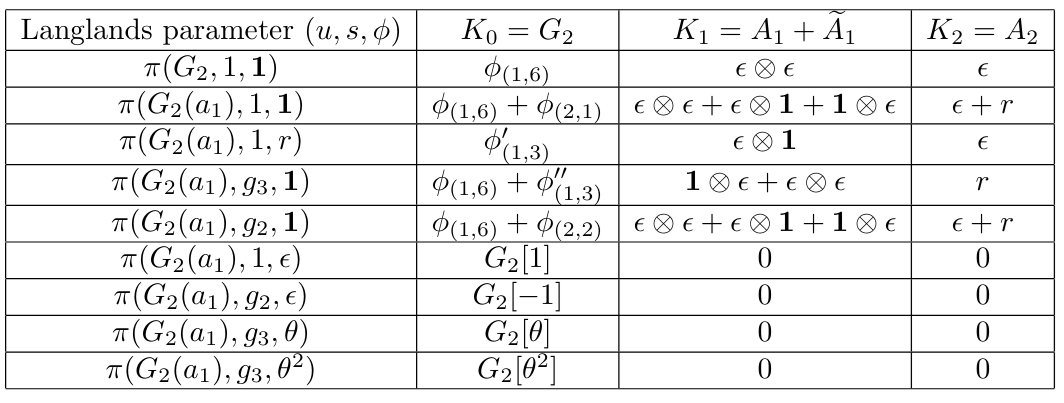
\includegraphics[scale=0.7]{subregular_element.png}
    \caption{Restrictions of $G_2$-representations $\pi(G_2(a_1),s,\phi)$}
    \label{tbl:G2_restriction_deleted}
\end{figure}
\fi

Twisting by the sign character yields the desired result. The proof of Conjecture \ref{conj:main} is now just a matter of putting all the pieces together. The parahoric restrictions of the virtual characters $\Pi(u,s,h)$ can be computed by linearity from the parahoric restrictions of the representations $\pi(u,s,\phi)$, which are given in Table \ref{tbl:G2_restriction}. 
\begin{table}[ht]
    \centering
    \begin{tabular}{|c|c|c|c|}
        \hline
        & $K_0\longrightarrow G_2$ & $K_1\longrightarrow A_1\times\tilde{A}_1$ & $K_2\longrightarrow A_2$ \\\hline
        $\Pi(G_2,1,1)$ & $\phi_{1,6}$ & $\epsilon\boxtimes\epsilon$ & $\epsilon$ \\\hline
        $\Pi(G_2(a_1),1,1)$ & $\phi_{2,1}+G_2[1]+2\phi_{1,3}'+\phi_{1,6}$ & $\mathbf{1}\boxtimes\epsilon+3\epsilon\boxtimes\mathbf{1}+\epsilon\boxtimes\epsilon$ & $3\epsilon+r$ \\\hline
        $\Pi(G_2(a_1),1,g_2)$ & $\phi_{2,1}-G_2[1]+\phi_{1,6}$ & $\mathbf{1}\boxtimes\epsilon+\epsilon\boxtimes\mathbf{1}+\epsilon\boxtimes\epsilon$ & $\epsilon+r$ \\\hline
        $\Pi(G_2(a_1),g_2,1)$ & $\phi_{2,1}+\phi_{2,2}+G_2[-1]+\phi_{1,6}$ & $\mathbf{1}\boxtimes\epsilon+\epsilon\boxtimes\mathbf{1}+\epsilon\boxtimes\epsilon$ & $\epsilon+r$ \\\hline
        $\Pi(G_2(a_1),1,g_3)$ & $\phi_{2,1}+G_2[1]-\phi_{1,3}'+\phi_{1,6}$ & $\mathbf{1}\boxtimes\epsilon+\epsilon\boxtimes\epsilon$ & $r$ \\\hline
        $\Pi(G_2(a_1),g_3,1)$ & $\phi_{1,3}''+G_2[\theta]+G_2[\theta^2]+\phi_{1,6}$ & $\mathbf{1}\boxtimes\epsilon+\epsilon\boxtimes\epsilon$ & $r$ \\\hline
        $\Pi(G_2(a_1),g_2,g_2)$ & $\phi_{2,1}+\phi_{2,2}-G_2[-1]+\phi_{1,6}$ & $\mathbf{1}\boxtimes\epsilon+\epsilon\boxtimes\mathbf{1}+\epsilon\boxtimes\epsilon$ & $\epsilon+r$ \\\hline
        $\Pi(G_2(a_1),g_3,g_3)$ & $\phi_{1,3}''+\theta G_2[\theta]+\theta^2 G_2[\theta^2]+\phi_{1,6}$ & $\mathbf{1}\boxtimes\epsilon+\epsilon\boxtimes\epsilon$ & $r$ \\\hline
        $\Pi(G_2(a_1),g_3,g_3^{-1})$ & $\phi_{1,3}''+\theta^2 G_2[\theta]+\theta G_2[\theta^2]+\phi_{1,6}$ & $\mathbf{1}\boxtimes\epsilon+\epsilon\boxtimes\epsilon$ & $r$ \\\hline
    \end{tabular}
    \caption{Restrictions of $G_2$-representations $\pi(G_2(a_1),s,\phi)$}
    \label{tbl:G2_restriction}
\end{table}

Finally, Lusztig's nonabelian Fourier transform acts trivially on every representation, except for the $G_2(\FF_q)$ family 
$$\{\phi_{2,1},\phi_{1,3}',G_2[1],\phi_{2,2},G_2[-1],\phi_{1,3}'',G_2[\theta],G_2[\theta^2]\},$$
where the action is given by the $8\times 8$ matrix
\begin{figure}[!ht]
    \centering
    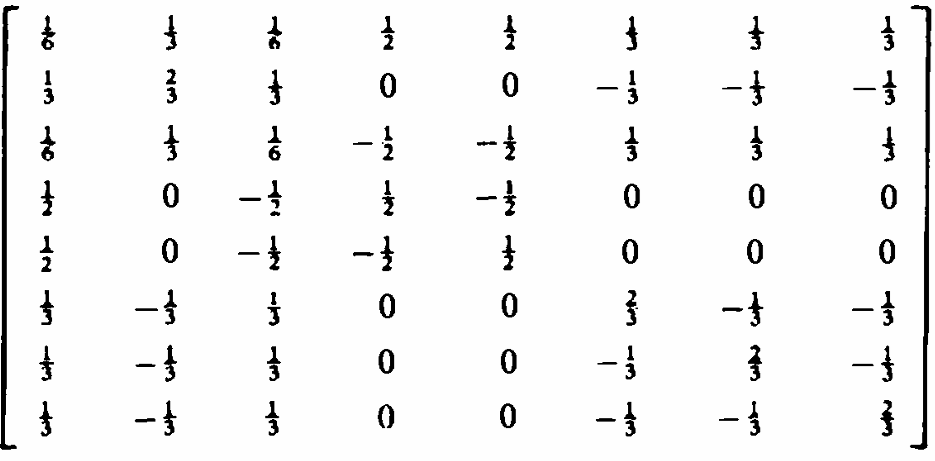
\includegraphics[scale=0.4]{fourier transform matrix.png}
\end{figure}
It is now a routine calculation to see that the square in Conjecture \ref{conj:main} commutes.